\section{粒子的波动性}

\begin{quotation}
“粒子是一种观念形态的概念,它产生于我们为了表示事物在给定时刻处于空间某点的定位的思想。” \qquad 德布罗意
\end{quotation}

\subsection{物质波的概念}

\begin{figure}[h]
\begin{center}
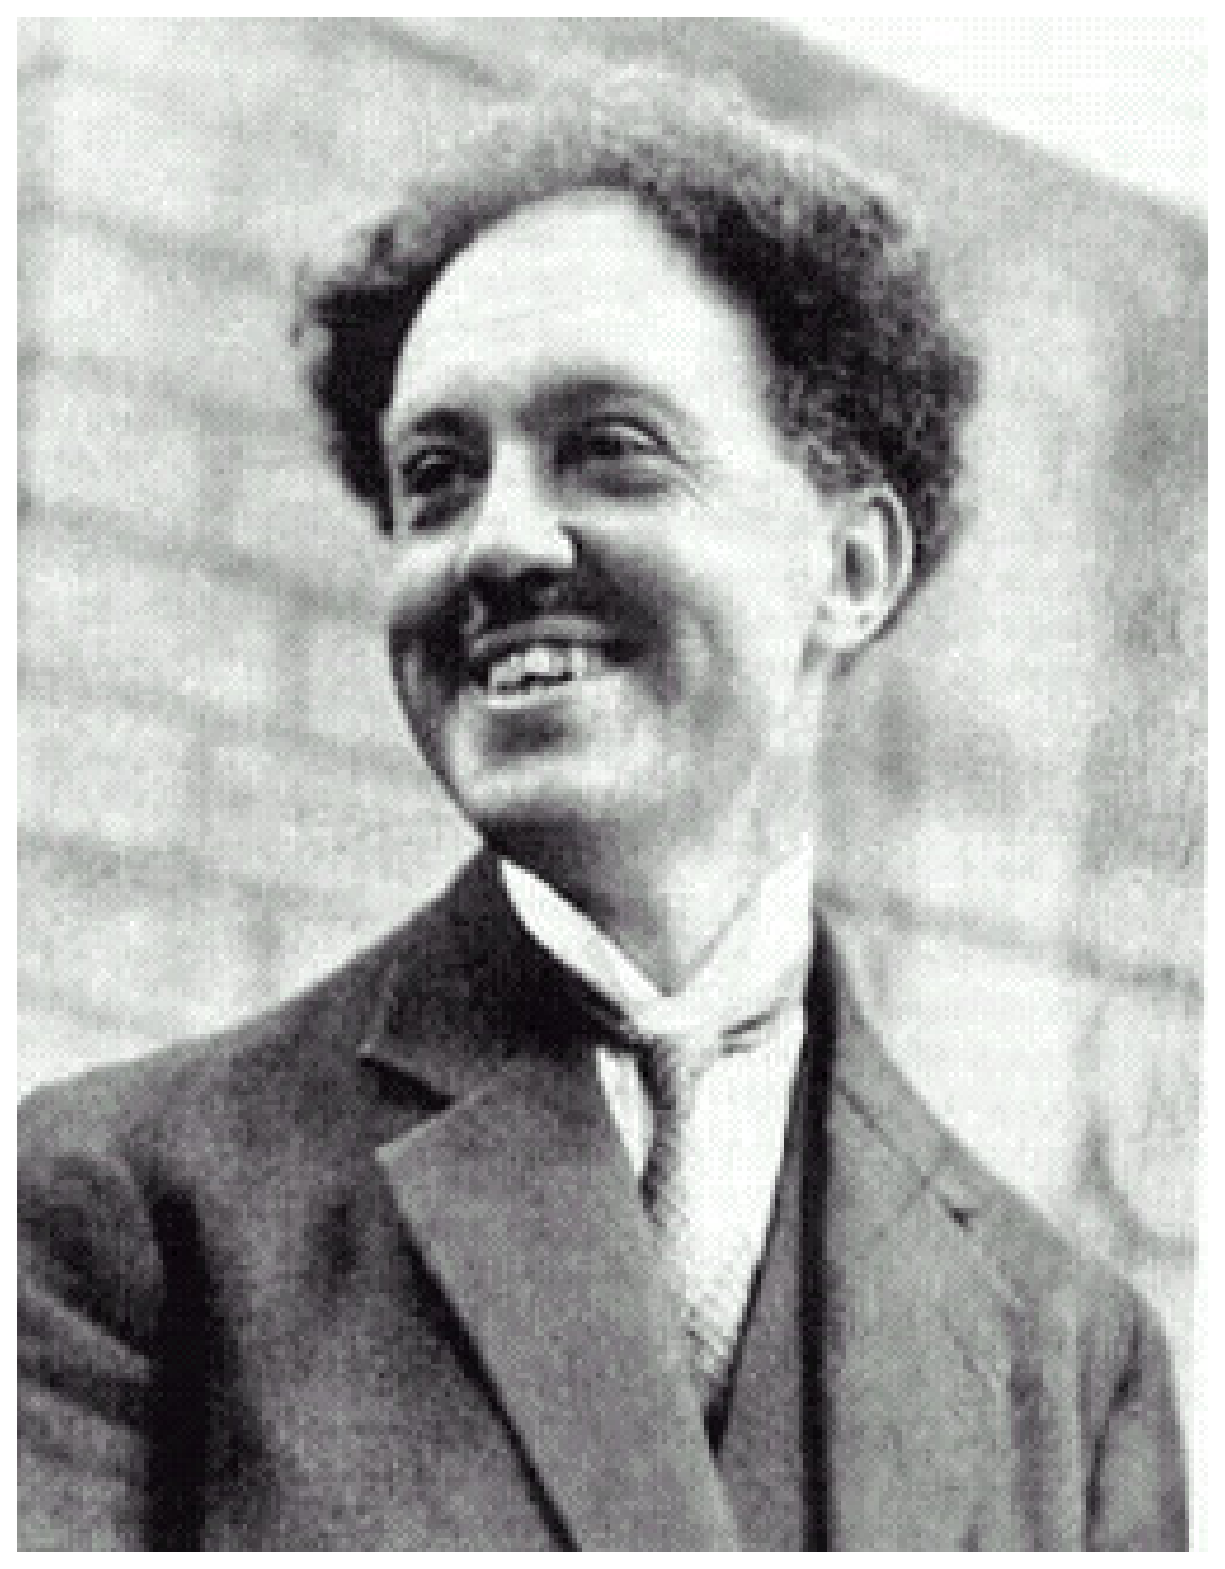
\includegraphics[clip,width=6cm]{Duality/debroglie.ps}
\caption{德布罗意}
\end{center}
\end{figure}

\subsubsection*{宏观物理学与微观物理学的对立}

玻尔的原子理论向我们揭示,微观尺度的物理学规律与宏观尺度的经典物理学规律是不同的。
光波在宏观尺度是经典的波动(连续形式的运动),而在微观尺度则体现为波粒二象性(wave-particle
duality), 既有波动性又有粒子性。

1923年,德布罗意(de
Broglie)提出:对物质粒子而言在微观尺度同样应具有``波粒二象性''的假设,
即在微观尺度,电子会体现出波动性,
有干涉、衍射现象,可以用波动方程表示微观粒子的运动。

\index{Quantization of angular momentum: 角动量量子化}

德布罗意受玻尔理论启发,``角动量量子化''为原子的定态运动引入了整数$n$,而在经典物理学中,``驻波''也对应整数$n$。
玻尔理论中角动量量子化:

$L = mvr = n\hbar $ $\Rightarrow$ $pr = \frac{{nh}}{{2\pi }}$
$\Rightarrow$ $2\pi r = \frac{{nh}}{p}$

\begin{figure}[h]
\begin{center}
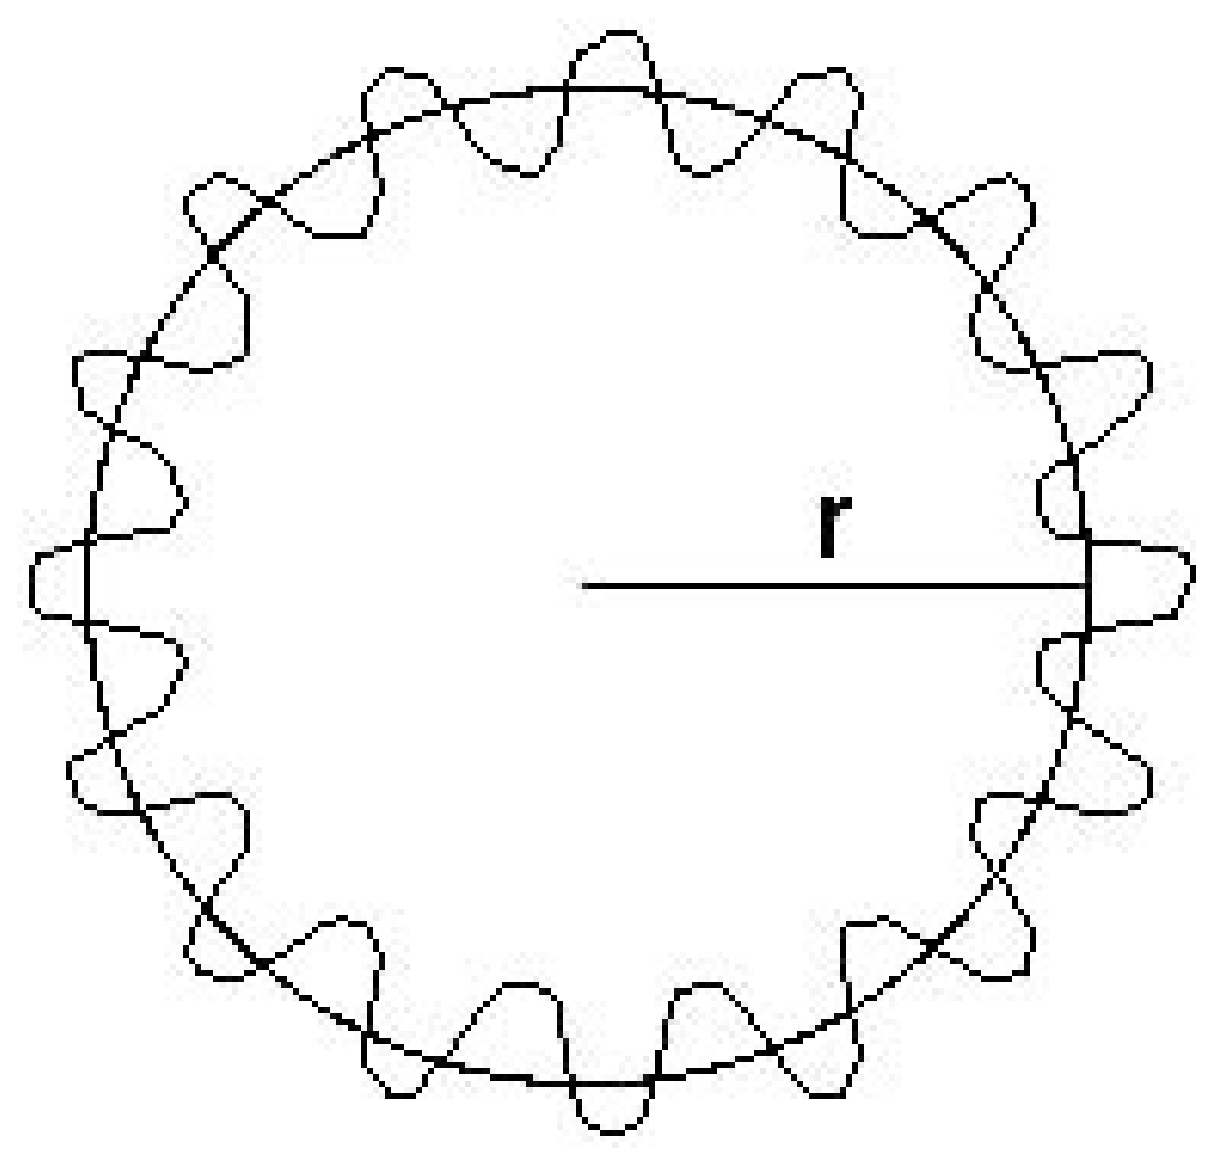
\includegraphics[clip,width=6cm]{Duality/5-1.ps}
\caption{电子在半径为r圆轨道上的驻波}
\end{center}
\end{figure}

\index{Standing wave: 驻波}

如果把玻尔理论中的定态对应为电子在圆轨道上的驻波,则:$2\pi r = n\lambda  = n\frac{h}{p}$
(即:电子围绕原子核运动一周,相位正好变化 的整数倍,同位相波动相长。)

得到德布洛意关系式:

\begin{equation}\label{5-1}
\lambda  = \frac{h}{p}
\end{equation}


这样就把粒子的特征:动量($p$)与波动的特征:波长($\lambda$ )联系了起来。

利用普朗克量子化条件也可以把粒子的能量与波动的频率联系起来:$\nu  =
\frac{\varepsilon }{h}$, 形式上与表示光的波粒二象性所用方程一样,
$\lambda ,\nu $ 分别是物质波的波长和频率。
(由于光子静质量为$0$,也可把物质波看作是``波粒二象性''由质量为$0$情形向质量不为$0$情形的推广)

这样微观粒子的运动状态可用波动方程表示,如对自由粒子,具有确定的能量$E$和动量$p$,所以对应描写波动的函数为一个平面波(plane
wave): $\psi  = A\cos \left[ {k \cdot r - \omega t} \right],k =
\frac{{2\pi }}{\lambda }\hat n,\omega  = 2\pi \nu $ ,这里$\hat
n$是波动传播方向(粒子运动方向)的单位矢量。

这个波函数(wave function)也可写为复数形式:

\begin{equation}
\psi  = Ae^{i(k \cdot r - \omega t)} = Ae^{\frac{i}{\hbar }(p \cdot
r - Et)}
\end{equation}

这种波称为德布罗意波或物质波(matter wave)。

\textbf{例1:相对论情形和非相对论情形下的德布罗意关系式:}

对于非相对论情形,$\varepsilon _k  = \frac{{p^2 }}{{2m_0 }}$,$p = \sqrt {2m_0 \varepsilon _k } $

相对论情形:$E^2  = p^2 c^2  + m_0 ^2 c^4 $,


$p = \frac{1}{c}\sqrt {E^2  - m_0 ^2 c^4 }  = \frac{1}{c}\sqrt
{\left( {m_0 c^2  + \varepsilon _k } \right)^2  - m_0 ^2 c^4 } $

$ = \frac{1}{c}\sqrt {\varepsilon _k ^2  + 2m_0 c^2 \varepsilon _k }
 = \sqrt {2m_0 \varepsilon _k  + \left( {{\textstyle{{\varepsilon
_k } \over c}}} \right)^2 } $

所以当$\varepsilon _k  \ll c$时,即得到非相对论情形下的公式。

$\nu  = \frac{E}{h} = \frac{{\sqrt {p^2 c^2  + m_0 ^2 c^4 } }}{h} =
\frac{{m_0 c^2 }}{h}\left( {1 + \frac{1}{2}\left( {\frac{{p^2 c^2
}}{{m_0 ^2 c^4 }}} \right) + ...} \right) $

$ = \frac{{m_0 c^2 }}{h}\left( {1 + \frac{{p^2 }}{{2m_0 ^2 c^2 }} +
...} \right) = \frac{1}{h}\left( {m_0 c^2  + \frac{{p^2 }}{{2m_0 }}
+ ...} \right)$

由于能量只有相对变化$\Delta E$才有意义(即能量的绝对值在物理上是没有意义的,它依赖于``零能量值''的选取),$h\nu  = \Delta E = E_2  - E_1 $ ,可将常数项$m_0 c^2 $抵消,此时相对论形式的关系退化为非相对论情形:$\nu  = \frac{{\varepsilon _k }}{h}$,$\varepsilon _k $就是非相对论粒子的动能。

德布罗意频率本身不是一个可观测量,只有德布罗意波长具有物理意义。

\textbf{例2:为什么物质的波动性在宏观尺度不显现}

由$\lambda  = \frac{h}{p}$,原因是普朗克常数太小($h = 6.6 \times 10^{ - 34} J \cdot s$),而宏观尺度的运动动量太大。如考虑一个50kg的人运动速度是0.5m/s,则可计算出对应物质波波长为:
$\lambda  = \frac{h}{p} = \frac{{6.6 \times 10^{ - 34} J \cdot s}}{{\left( {50} \right)\left( {0.5} \right)\left( {kg \cdot m/s} \right)}} = 2.6 \times 10^{ - 35} m$。
显然太小,难以引起可以观察的物理效应。

$p = \sqrt {2mE} $, 要减小宏观尺度运动的动量, 必须减小动能$E$,
但从物理上考虑$E$不可能减小到比热运动能量$k_B T$更小,
所以必须减小质量。质量的减小对应于尺度的减小。只有把物体尺度减小到微观尺度,
才可能出现较大的物质波波长 $\lambda$,从而引起可以观察到的物理效应。


\subsection{戴维孙-革末实验}

考虑电子被$V$伏特电场加速, $\lambda  = \frac{h}{p} =
\frac{h}{{\sqrt {2m_e E} }} = \frac{h}{{\sqrt {2m_e eV} }} \approx
\frac{{12.27}}{{\sqrt V }} {\AA}$.

当$V=150$伏时,$\lambda  = 1 {\AA}$。
如果用间距为1埃数量级的光栅,则应观察到入射电子的干涉条纹,人工加工这么小的尺度显然是困难的,
但自然界中单晶原子间距恰好大约是1埃,所以单晶可用作验证物质波假说的光栅。

\begin{figure}[ht]
\begin{center}
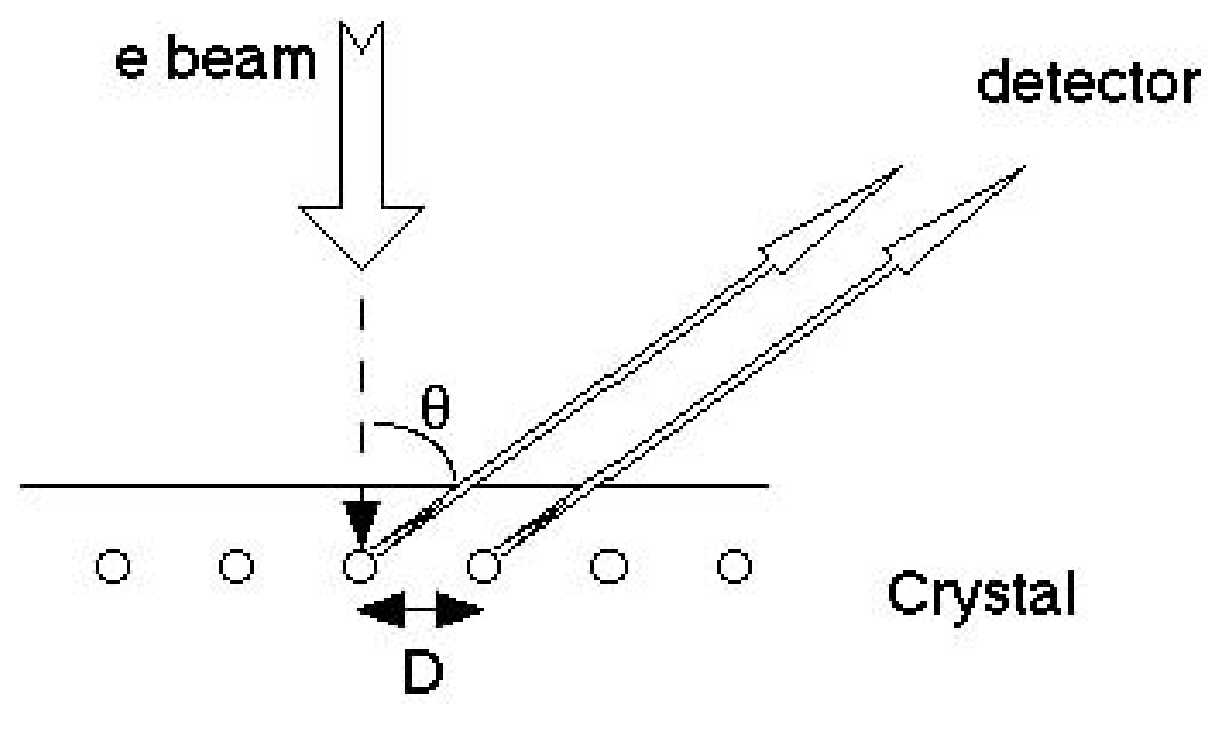
\includegraphics[clip,width=7cm]{Duality/5-2.ps}
\caption{电子被单晶衍射}
\end{center}
\end{figure}


对某晶面干涉相长条件:

\begin{center}
\begin{equation}
\label{bragg condition}
    D\sin \theta  = n\lambda
\end{equation}
\end{center}

$D$为晶面上相临原子间距,也叫布拉格条件(Bragg condition), 注意:
因角度$\theta$的选取不同, 布拉格公式的具体形式可能会有不同。

\index{Bragg's formula: 布拉格公式}

\index{Davisson–Germer experiment: 戴维孙-革末实验}

1925年,戴维孙(Davisson)和革末(Germer)在做电子在镍(Ni)单晶上散射实验时,第一次观察到电子在晶体中的衍射现象。
散射电子强度在特定方向$\theta$出现极大值。
实验证明微观粒子确实具有波动性质,所以和光一样,物质粒子也具有``波粒二象性''。

\index{Wave-particle duality: 波粒二象性}


\begin{figure}[ht]
\centering
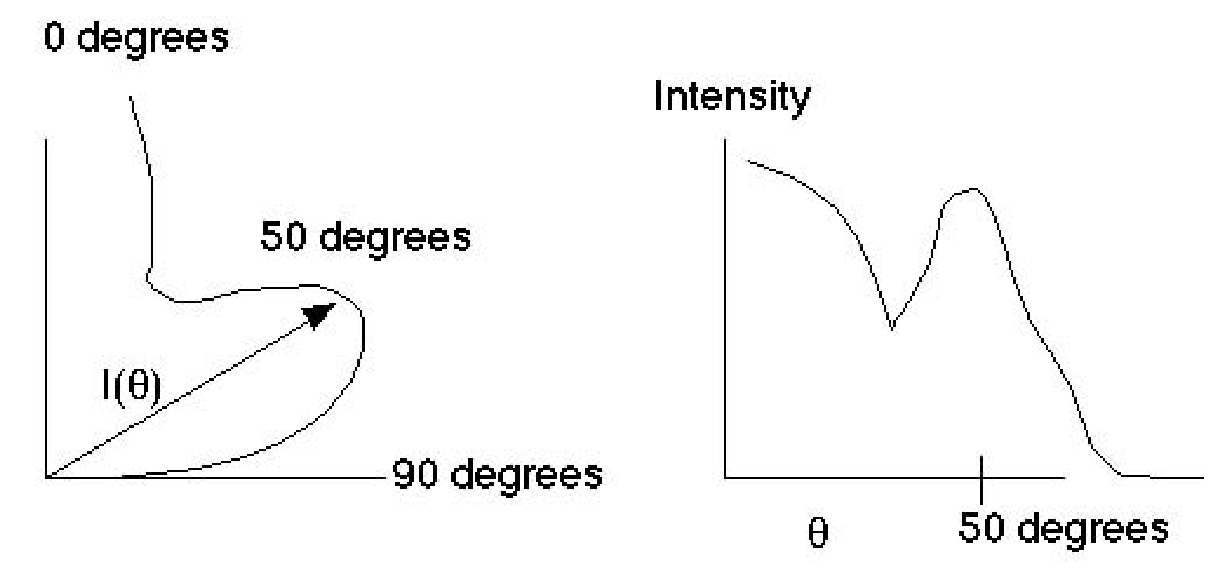
\includegraphics[width=8cm]{Duality/5-3.ps}
\caption{电子在单晶中的衍射图样}
\end{figure}



\subsection{电子的双缝干涉实验}

为说明电子的波粒二象性,我们做``电子双缝干涉''(double-slit
experiment)的理想实验\footnote{这个理想实验在费曼物理学讲义中有详细讨论,
最近确实有实验物理学家在实验室里实现了``电子的双缝干涉'',请参考:

\url{http://physicsworld.com/cws/article/print/2002/sep/01/the-double-slit-experiment}

}。

\index{Double-slit experiment: 双缝实验}

(1)一束电子通过双缝:

\begin{figure}[ht]
\begin{center}
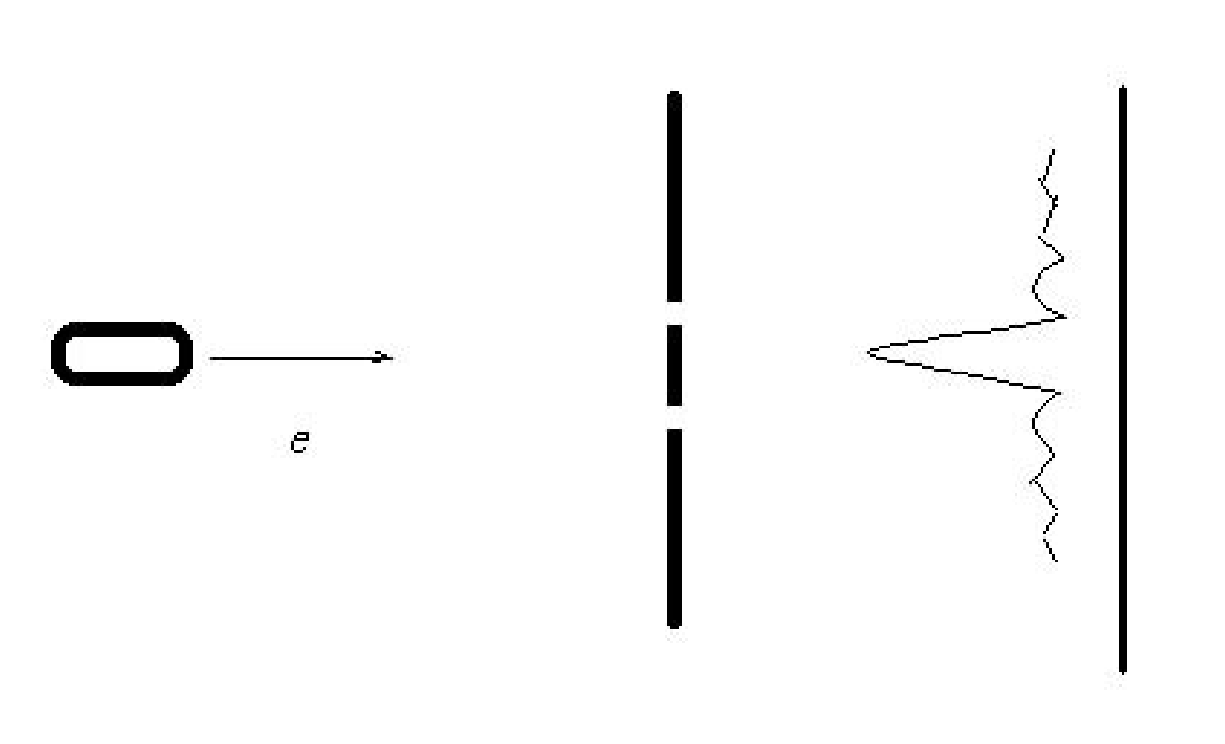
\includegraphics[clip,width=6cm]{Duality/5-4.ps}
\caption{一束电子通过双缝}\label{Duality/5-4-ps}
\end{center}
\end{figure}

在屏上可观察到干涉条纹,说明电子确实有波的性质。(如图\ref{5-4-ps})

问题:波动性质(干涉效应的出现)是电子的集体行为(不同电子间干涉)?
还是电子本身的性质(每个电子自己和自己发生干涉效应)?

(2)单电子干涉

\begin{figure}[ht]
\begin{center}
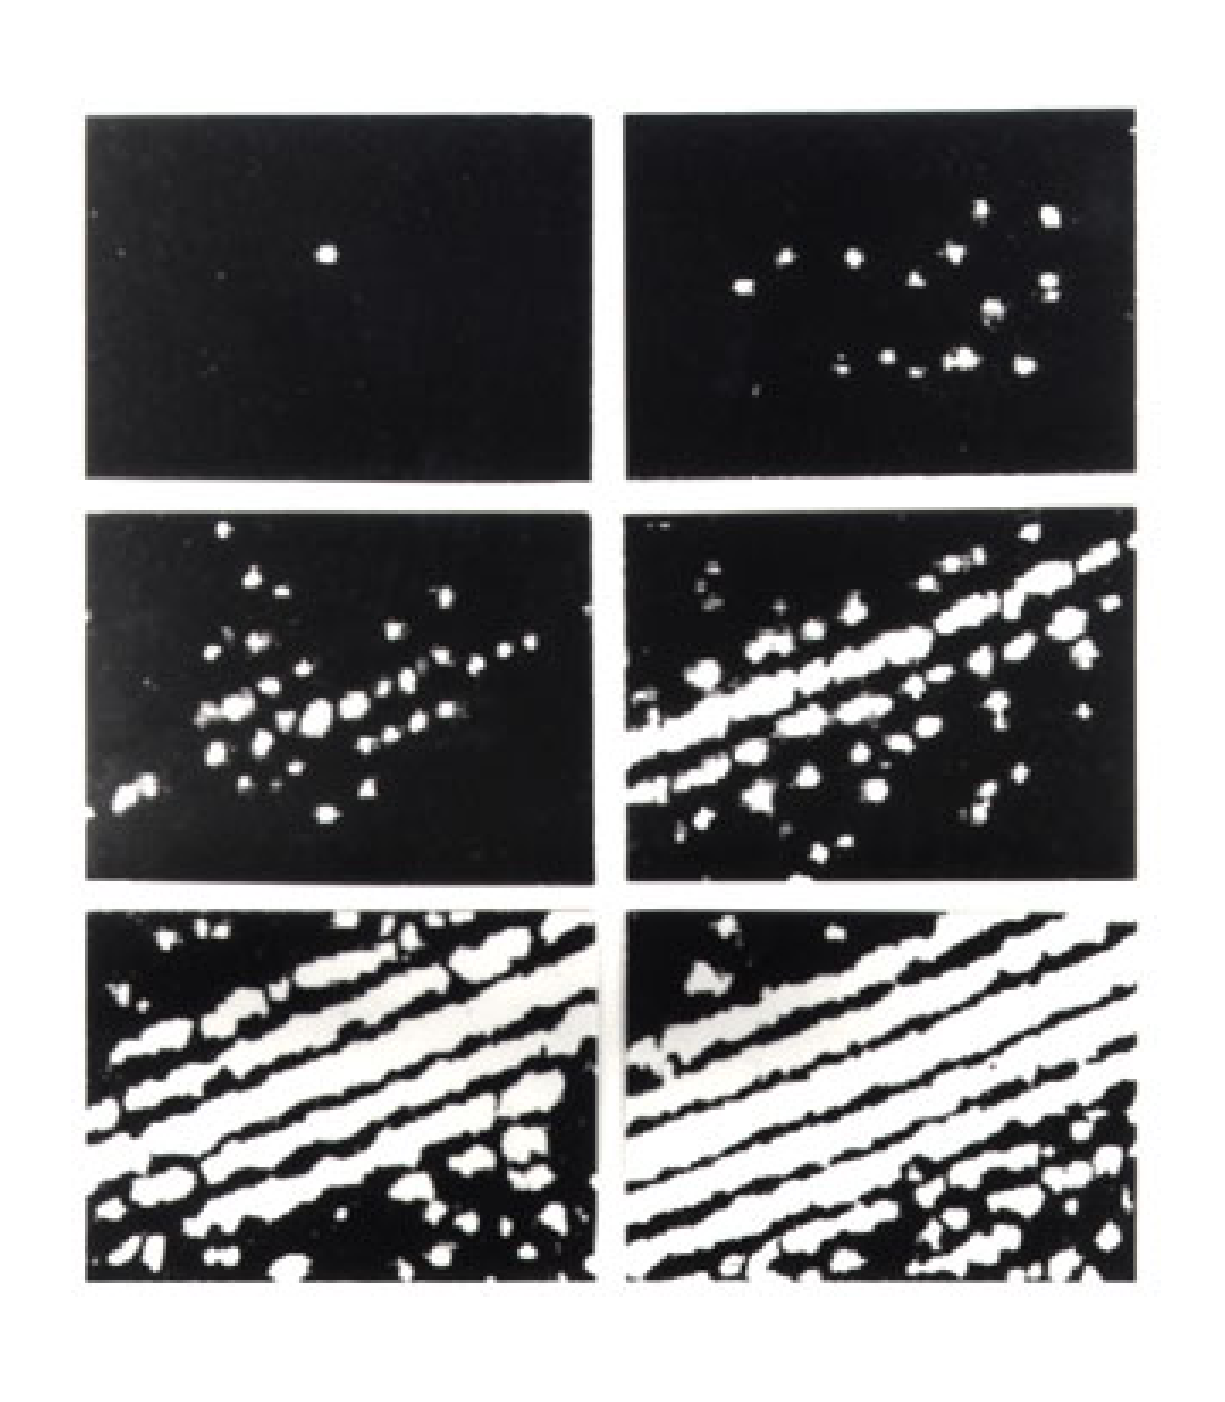
\includegraphics[clip,width=6cm]{Duality/double-slit.ps}
\caption{实验观察到的``单电子干涉''}\label{5-4-ps}
\end{center}
\end{figure}


为解决实验(1)所提出的问题,我们可以做单电子干涉实验,即让电子一个一个地穿过双缝,看会发生什么。

实验结果显示:

电子只在屏上一点被探测到,说明电子是穿过双缝之一,并没有``一分为二'',分别穿过两个缝(体现为粒子性)。
但电子在屏上出现的具体位置是没有规律的,若长时间观察,电子一个一个累计的效果是再次出现干涉条纹(体现为波动性)。
不同电子穿过双缝分别都是独立事件,每个电子在屏上出现的几率分布$P(x)$应是相同的。
单电子也体现出波动性,即波动性是微观粒子的本质属性,
或``波粒二象性''是微观粒子的本质属性。

(3)挡住一条缝

\begin{figure}[ht]
\begin{center}
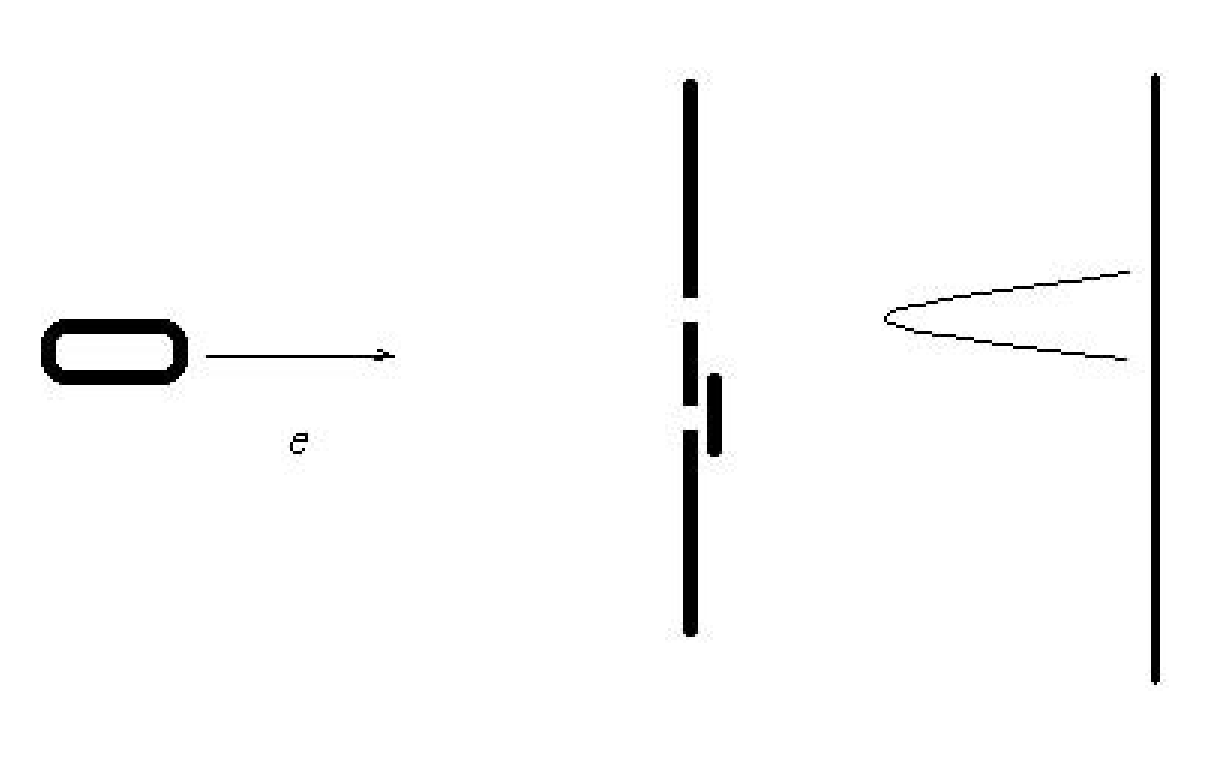
\includegraphics[clip,width=6cm]{Duality/5-5.ps}
\caption{挡住一条缝,干涉条纹消失}\label{5-5-ps}
\end{center}
\end{figure}

干涉条纹消失,电子集中在未遮挡缝延长方向上,表现为粒子性,如图\ref{5-5-ps}。(为叙述方便,我们先不考虑单缝衍射效应)

(4)控制开关,人为地遮挡两个缝中的任何一个

\begin{figure}[ht]
\begin{center}
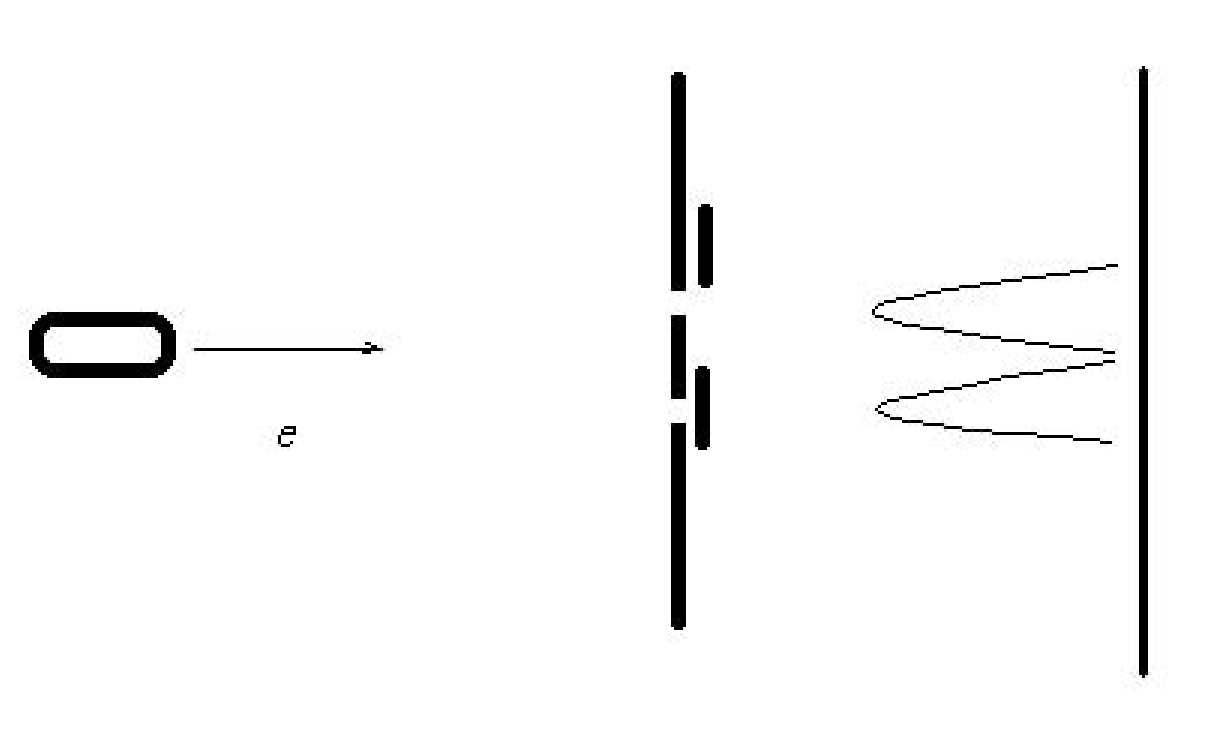
\includegraphics[clip,width=6cm]{Duality/5-6.ps}
\caption{人为地遮挡两个缝中的任何一个}\label{5-6-ps}
\end{center}
\end{figure}

我们任意地遮挡住两个缝中任何一个,遮挡顺序是无序的,但必须确定,即是人为可以控制的。
这时,干涉条纹消失,电子穿过双缝积累效果是电子集中在双缝方向分布,出现两个峰,如图\ref{5-6-ps},体现为粒子性。

(5)在``双缝''处分别安装测量装置,使之可以测量电子究竟是从哪个缝穿过的。

这种可以测量电子位置的装置是一种``理想装置'',它的作用就是获取电子的位置信息,
至于它是如何实现的\footnote{我们可以使用光子来探测电子的位置,即在双缝两边各放一光源($P_1$, $P_2$)和一光探测器($D_1$, $D_2$)。
光源发出的光子打在经过狭缝的电子上,被散射出来由探测器记录,并给出信号。参考杨福家《原子物理学》第97页。},在这里我们并不关心。

实验结果是:如每个电子穿过哪条缝都被成功观测到,则干涉条纹消失。
电子穿过双缝积累效果是电子集中在双缝方向分布,出现两个峰。(体现为:粒子性)

实验(5)与实验(4)本质上是相同的,即系统是``单缝''而不是``双缝'',所以不会发生干涉。
一旦我们可以确认电子是由哪条单缝穿过的,另一条单缝对电子来说就是``不存在''的,即相当于另一条单缝被遮挡。

\subsection{海森堡不确定关系}

\begin{figure}[h]
\begin{center}
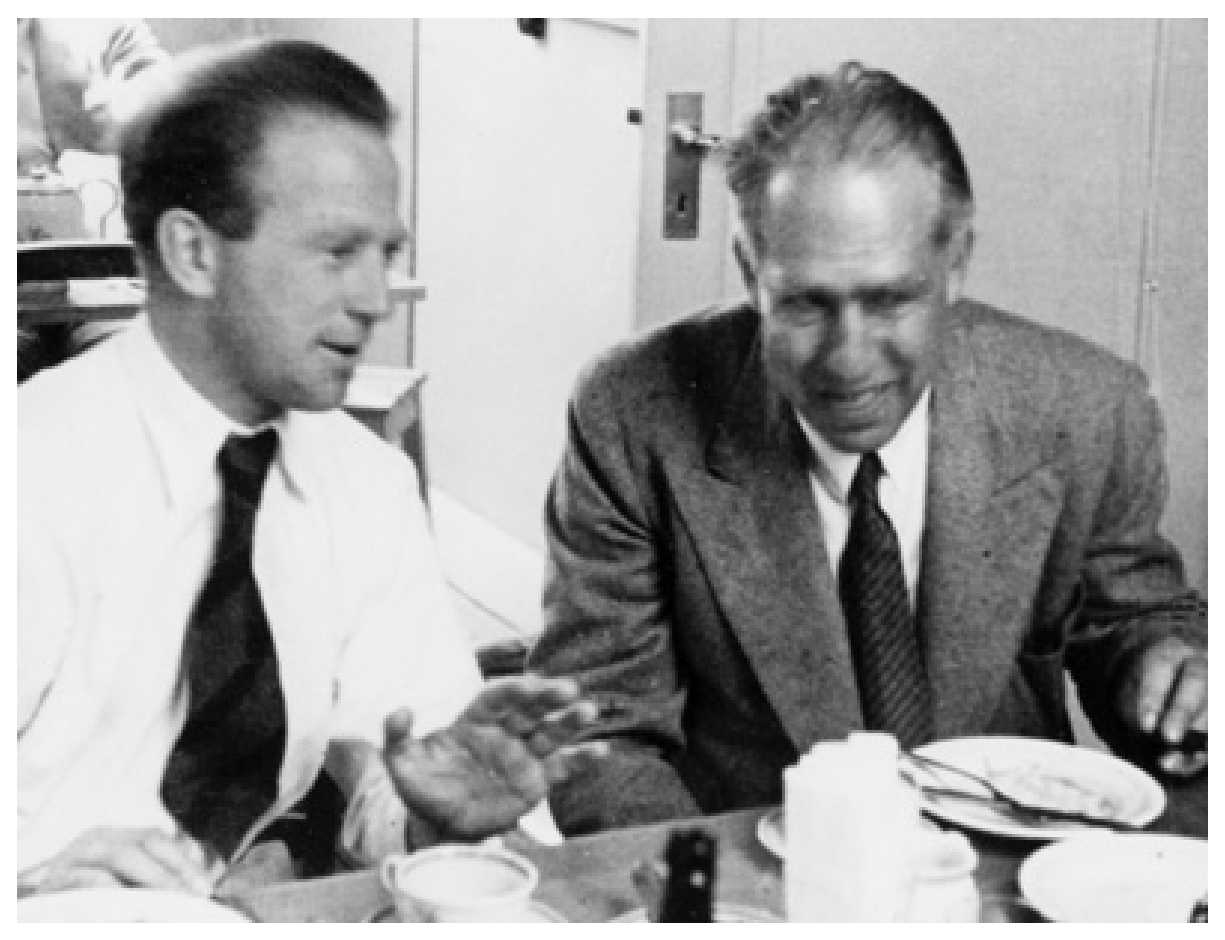
\includegraphics[clip,width=6cm]{Duality/bohr-hei.ps}
\caption{海森堡在哥本哈根与玻尔工作期间提出了不确定原理}
\end{center}
\end{figure}


\begin{figure}[ht]
\begin{center}
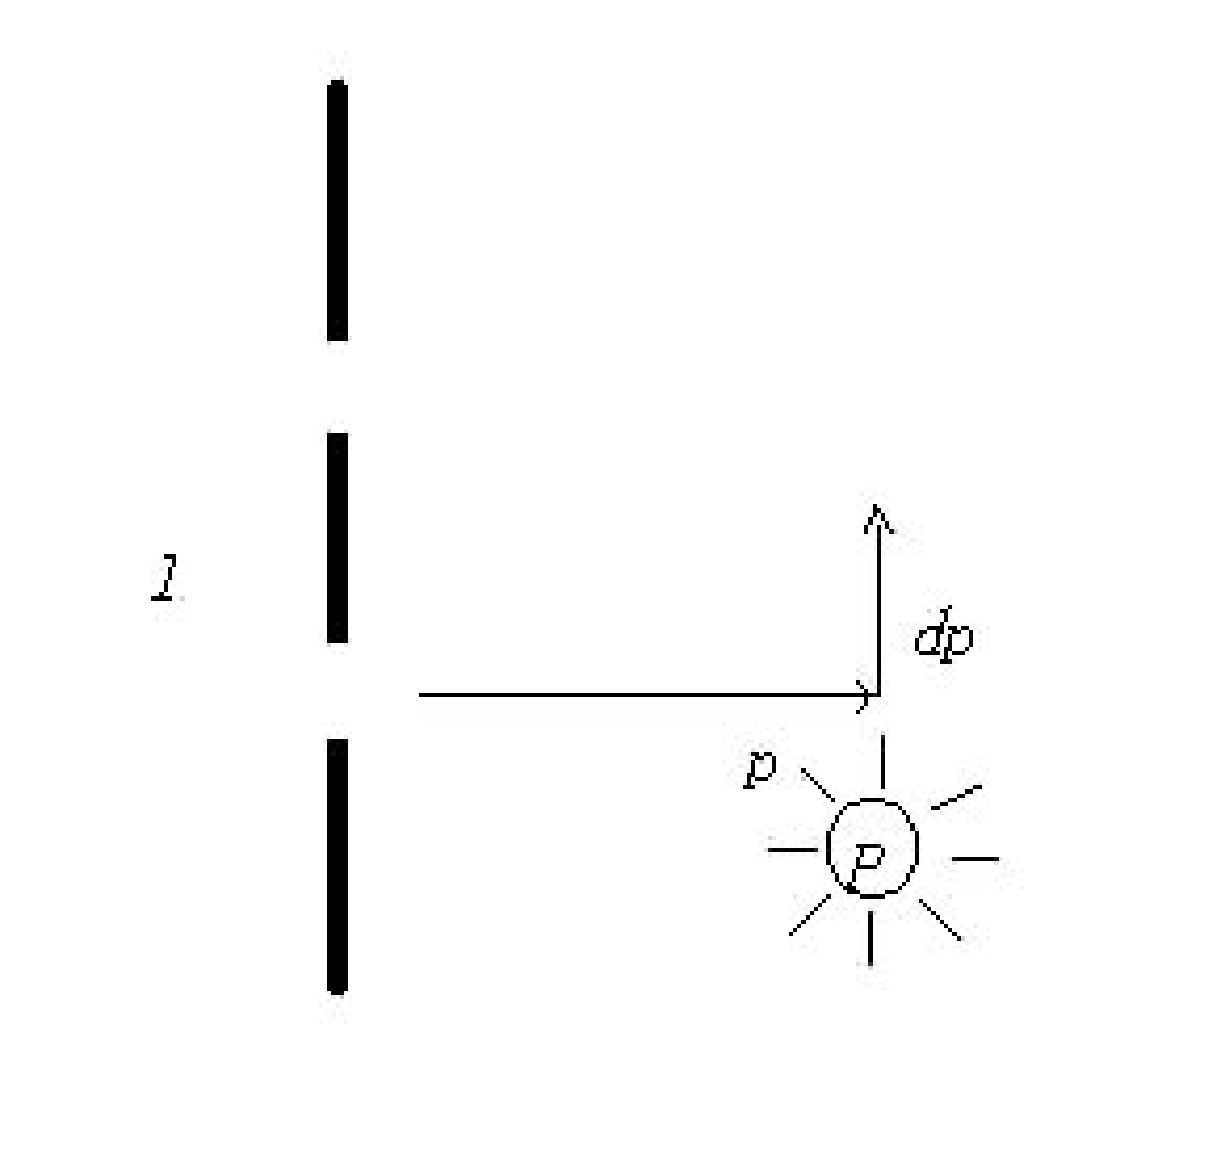
\includegraphics[clip,width=5cm]{Duality/5-7.ps}
\caption{测不准关系示意}\label{5-7-ps}
\end{center}
\end{figure}


不确定关系(uncertainty relation,
也叫测不准关系)是海森堡(Heisenberg)1927年首先提出的:

\index{Uncertainty principle: 不确定原理}

\begin{center}
\begin{eqnarray}
% \nonumber to remove numbering (before each equation)
  \Delta p_x \Delta x \ge h\\
  \Delta E\Delta t \ge h
\end{eqnarray}
\end{center}

不确定关系还有多种其他表示形式,这是其中最常用的两个。
不确定关系表明,微观粒子在客观上不能同时具有确定的坐标及相应确定的动量。

如图\ref{5-7-ps},考虑电子双缝干涉,两缝间距为$l$;
为测量电子是从哪个缝中射出,光源P发出的测量光子必须具备至少$l$的分辨本领,即:$\lambda
\le l$。 则测量光子至少具备动量:$p \ge \frac{h}{l}$。
测量光子转移给电子的动量为:$\Delta p \ge \frac{h}{l}$,
假设测量光子动量全部转移。所以光子对电子测量结果:$\Delta x =
l,\Delta p \ge \frac{h}{l}$, 即:$\Delta p_x \Delta x \ge
h$,这是不确定关系的粗略推导,严格证明我们将在后续的章节中给出。

\textbf{例3:谱线的自然宽度}

\begin{figure}[ht]
\begin{center}
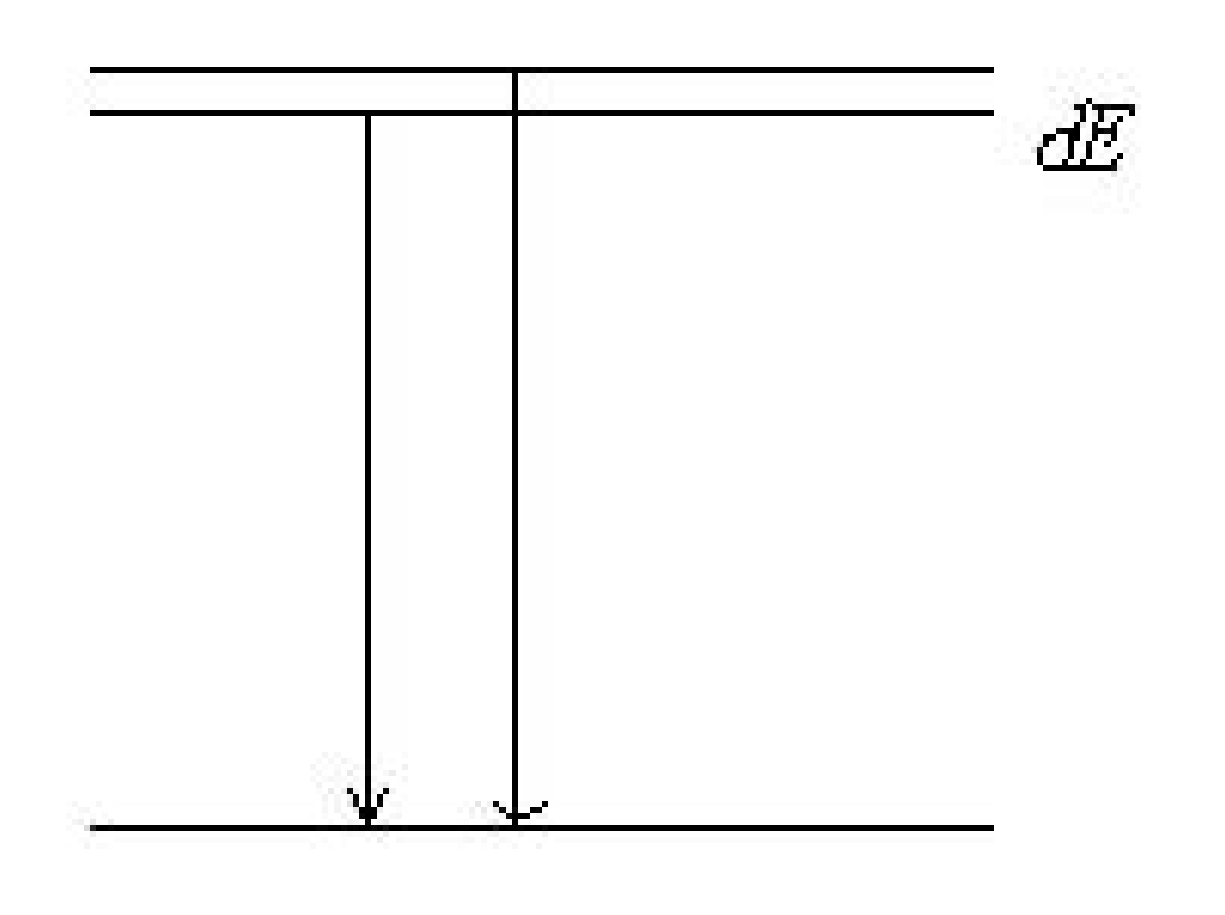
\includegraphics[clip,width=5cm]{Duality/5-8.ps}
\caption{谱线的自然宽度}\label{5-8-ps}
\end{center}
\end{figure}

\index{Natural width of spectral line: 谱线的自然宽度}

\index{Energy-Time Uncertainty Relation: 能量-时间不确定关系}

假设电子在激发态(能量较高的能级)具有一定寿命$\Delta
t$,即电子被激发到激发态后,再过$\Delta t$
跃迁回基态。这样激发态能量对应有一个不确定值$\Delta E \sim
\frac{h}{{\Delta t}}$。
这样谱线(对应由激发态跃迁到基态)将有一定宽度,不再是``绝对的线'',
这也常被表述为``能量-时间的不确定关系''(Energy-Time Uncertainty
Relation).\footnote{
``能量-时间不确定关系''和``动量-位置不确定关系''在物理上的解释是不同的.
根据量子力学的体系, 位置是算符, 时间只是参数, 而不是算符,
``动量-位置不确定关系''可由算符对易关系证明,
而``能量-时间不确定关系''则没有这样的证明,
``能量-时间不确定关系''的证明可在学习完量子力学中的``含时微扰''后再研究.}



\subsubsection{估算氢原子基态能}

利用不确定关系,我们可以做很多近似估算,比如我们可以估算氢原子的基态能量。
首先, 氢原子的哈密顿:$H = \frac{p^2}{2m} - \frac{e^2}{4 \pi
\epsilon_0 r}$

\index{Hydrogen atom: 氢原子}


考虑严格形式的不确定关系: $\Delta x \Delta p \ge \hbar /2$

在经典的意义下考虑电子的运动, 即电子围绕质子作圆周运动,
但根据不确定关系, 电子运动半径应存在最小值,
此时即对应氢原子的基态。这种方法不是量子力学地处理氢原子的一般性方法,
只能估算基态, 但无法计算激发态。

直接的估算是假设位置的不确定为:$\Delta r = a$,$\Delta p =
p$;因为研究的是基态,所以只需考虑等号,$a \cdot p =
\frac{\hbar}{2}$,$p=\frac{\hbar}{2a}$代入哈密顿中,得到能量的估计值:

\begin{equation*}
  E(a)=\frac{\hbar^2}{8 a^2 m} - \frac{e^2}{4 \pi \epsilon_0 a}
\end{equation*}

基态对应最低能量, 因此应有$\frac{\partial E(a)}{\partial a} |_{a_0}
= 0$,
然后把解出的$a_0$代入$E(a)$的表达式即为氢原子基态能的估算值$E(a_0)$。但这样估算出的氢原子基态能在数值上与严格解的结果并不相符。


如果假设$a \cdot p = \hbar$, 则能得到数值上正确的结果,
尽管利用不确定关系估算物理系统的基态能仅在定性上有意义,
但造成这一情况的原因仍值得思考。同样的做法,
对线性谐振子我们可以计算出定量上正确的结果,
而对氢原子而言就只能是定性的了?

以下,我们给出一种可能的解释,在经典图像下,氢原子中的电子围绕原子核运动,这是一个二维的运动。即应有:
$r^2 =x^2 + y^2$, $p^2 = p_x^2 + p_y^2$。

对$x$,$p_x$和$y$,$p_y$而言,应有:$\Delta x \Delta p_x \ge
\frac{\hbar}{2}$,$\Delta y \Delta p_y \ge \frac{\hbar}{2}$

那么:$\Delta r \Delta p = \sqrt {\Delta x^2 + \Delta y^2}
\sqrt{\Delta p_x^2 + \Delta p_y^2}$


考虑到$x$方向上的不确定度应该和$y$方向上的不确定度相等,
假设:$\Delta x^2 + \Delta y^2 = 2 \Delta x^2$,$\Delta p_x^2 +
\Delta p_y^2 =2 \Delta p_x^2$

那么:$\sqrt {\Delta x^2 + \Delta y^2} = \sqrt{2} \Delta
x$,$\sqrt{\Delta p_x^2 + \Delta p_y^2} = \sqrt{2} \Delta
p_x$,$\Delta r \Delta p = 2 \Delta x \Delta p_x = \hbar$

假设:$\Delta r =a$,$\Delta p = \frac{\hbar}{a}$, 那么:

\begin{equation*}
  E(a) = \frac{\hbar^2}{2m a^2} - \frac{e^2}{4 \pi \epsilon_0 a}
\end{equation*}



$\partial_a E(a) |_{a_0}= - \frac{\hbar^2}{m a_0^3} + \frac{e^2}{4
\pi \epsilon_0 a_0^2} = 0$,解出:$a_0 = \frac{4 \pi \epsilon_0
\hbar^2}{me^2}$,这个结果与用玻尔模型计算出的第一玻尔半径相同。考虑到精细结构常数:$\alpha
= \frac{e^2}{4 \pi \epsilon_0 \hbar c} = \frac{1}{137}$,$a_0 =
\frac{\hbar}{mc \alpha}$。

代入$E(a)$:$E(a_0) = - \frac{m c^2
\alpha^2}{2}$,此即玻尔模型计算出的氢原子基态能。考虑到电子质量为$mc^2
= 511 \text{keV}$,计算出$E(a_0) = -13.6
\text{eV}$。(玻尔模型计算出的能级为:$E_n = - \frac{13.6
\text{eV}}{n^2}$,如果原子核上有$Z$个质子,则$E_n = - \frac{13.6
Z^2}{n^2} \text{eV}$)




\subsection{对物质波的理解}

\subsubsection*{波包}

\index{Wave packet: 波包}

``如何理解物质波''是量子力学中的关键问题。德布洛意把物质波理解为波包(wave
packet)。(或者说:他把粒子理解为波包,这样波粒二象性自然可以在波包概念上达到统一)

\index{Matter wave: 物质波}

物质波可以用波函数表示,如自由粒子可以用单色平面波: 

\begin{equation}
\psi _k (x,t) = A \exp \left[ {i(kx - \omega t)} \right]
\end{equation}

单色平面波在空间是无限扩展的。我们定义相速度$v_p$(phase velocity),即固定相位$\varphi_0 = kx - \omega t$。对$\varphi_0$求微分:

\begin{equation}
d \varphi_0 = k dx - \omega dt  = 0
\end{equation}

相速度$v_p$是:

\begin{equation}
v_p  = \frac{{dx}}{{dt}} = \frac{\omega }{k}
\end{equation}

实际问题中经常碰到的是波包(wave packet),即波动在有限空间中分布。
根据频谱分析(Fourier分析),波包总可以表示为不同波矢平面波的叠加,即:

\begin{equation}
\psi (x,t) = \frac{1}{{\sqrt {2\pi } }}\int_{ - \infty }^\infty  {A (k)\exp \left[ {i(kx - \omega t)} \right]dk} 
\end{equation}

频率和波矢的函数叫色散关系(Dispersion relation):$\omega  = \omega (k)$,那么:

\begin{equation}
\psi (x,t) = \frac{1}{{\sqrt {2\pi } }}\int_{ - \infty }^\infty  {A (k)\exp \left[ {i(kx - \omega (k)t} \right]dk} 
\end{equation}

考虑最简单的情况,即两列频率、波矢相近的单色平面波:

\begin{equation}
\left\{ \begin{array}{l}
 \psi _1  = A\exp \left[ {i(k_1 x - \omega _1 t)} \right] \\
 \psi _2  = A\exp \left[ {i(k_2 x - \omega _2 t)} \right] \\
 \end{array} \right.
\end{equation}

相互叠加:

\begin{equation*}
\psi  = \psi _1  + \psi _2  = A \left( e^{i(k_1 x - \omega _1 t)} + e^{i(k_2 x - \omega _2 t)} \right)
\end{equation*}

利用:$e^{iA}  + e^{iB}  = e^{i(A + B)/2} e^{i(A - B)/2}  + e^{i(A + B)/2} e^{i(B - A)/2} \\ = e^{i(A + B)/2} \left[ {e^{i(A - B)/2}  + e^{ - i(A - B)/2} } \right] = 2\cos ({\textstyle{{A - B} \over 2}})e^{i(A + B)/2} $

\begin{equation}
\psi  = 2A\cos \frac{{\Delta kx - \Delta \omega t}}{2}\exp \left[ {i\left( {kx - \omega t} \right)} \right],
\end{equation}

这里:

\begin{eqnarray*}
\Delta k &=& k_1  - k_2 \\
\Delta \omega &=& \omega _1  - \omega _2 \\
k &=& \frac{{k_1  + k_2 }}{2} \\
\omega &=& \frac{{\omega {}_1 + \omega _2 }}{2}
\end{eqnarray*}

由于$k_1$,和$k_2$很接近,$\Delta k$对应的是一个振荡很舒缓的波动,而$k$对应的是一个很激烈的波动,这两个波动“乘”在一起,相对舒缓的波动对应的就是$\psi$的轮廓或包络线,即波包的形状:

\begin{equation}
2A\cos \left( {\frac{{\Delta k \cdot x - \Delta \omega  \cdot t}}{2}} \right)
\end{equation}

波包的速度就是这个轮廓或包络线运动的速度:$\frac{{\Delta \omega }}{{\Delta k}}$,即群速度$v_g$(group velocity):

\begin{equation}
v_g  = \frac{{d\omega }}{{dk}}
\end{equation}

例如:物质波(自由粒子非相对论情形):$\hbar \omega  = \frac{{(\hbar k)^2 }}{{2m}},\omega  = \frac{{\hbar k^2 }}{{2m}}$,群速度:$v_g  = \frac{{d\omega }}{{dk}} = \frac{{\hbar k}}{m}$ 对应的才是粒子运动的速度,而相速度:$v_p  = \frac{\omega }{k} = \frac{{\hbar k}}{{2m}}$,则不是粒子运动速度。

真空中的电磁波:$\omega  = c k  = 2\pi c/\lambda $,$v_p  = v_g  = c$。

\textbf{例4:求相对论粒子德布洛意波对应的相速度,群速度。}

由德布洛意关系:$\lambda  = \frac{h}{p} = \frac{{h\sqrt {1 - (v/c)^2 } }}{{m_0 v}}$,所以:
$k = \frac{{2\pi }}{\lambda } = \frac{{2\pi m_0 v}}{{h\sqrt {1 - (v/c)^2 } }}$

$\nu  = \frac{E}{h} = \frac{{mc^2 }}{h} = \frac{{m_0 c^2 }}{{h\sqrt {1 - (v/c)^2 } }}$,所以:
$\omega  = \frac{{2\pi m_0 c^2 }}{{h\sqrt {1 - (v/c)^2 } }}$

相速度:$v_p  = \frac{\omega }{k} = \frac{{2\pi m_0 c^2 }}{{h\sqrt
{1 - (v/c)^2 } }} \cdot \frac{{h\sqrt {1 - (v/c)^2 } }}{{2\pi m_0
v}} = \frac{{c^2 }}{v}$

\index{Phase velocity: 相速度}

显然$\frac{{c^2 }}{v} > c$,是否违背相对论呢?相速度是否可用作信息传递的速度?

群速度:$v_g  = \frac{{d\omega }}{{dk}} = \frac{{d\omega /dv}}{{dk/dv}}$

$\frac{{d\omega }}{{dv}} =  - \frac{{2\pi m_0 c^2 }}{{2h}} \cdot \frac{{ - 2(v/c^2 )}}{{\left( {1 - (v/c)^2 } \right)^{3/2} }} = \frac{{2\pi m_0 v}}{{h\left( {1 - (v/c)^2 } \right)^{3/2} }}$

$\frac{{dk}}{{dv}} = \frac{{2\pi m_0 h\sqrt {1 - (v/c)^2 }  - 2\pi m_0 vh({\textstyle{1 \over 2}})\left( {1 - (v/c)^2 } \right)^{ - 1/2} ( - 2)(v/c^2 )}}{{h^2 \left( {1 - (v/c)^2 } \right)}}$,继续化简:

$\frac{{dk}}{{dv}} = \frac{{2\pi m_0 \left( {1 - (v/c)^2 } \right) + 2\pi m_0 (v/c)^2 }}{{h\left( {1 - (v/c)^2 } \right)^{3/2} }} = \frac{{2\pi m_0 }}{{h\left( {1 - (v/c)^2 } \right)^{3/2} }}$

所以:$v_g  = \frac{{d\omega /dv}}{{dk/dv}} = v$,即在相对论情形下粒子运动速度也对应于波包的群速度。

\index{Group velocity: 群速度}


计算表明波包形状随时间改变,即随着时间的变化,波包是不稳定的,会逐渐扩散出去\footnote{参考曾谨言《量子力学 卷I》第721页},就象我们在池塘里激起一朵水花,
这个波动会逐渐扩散开去,以致最后消失。所以,如果我们把粒子(电子)理解为波包,就会得出粒子是不稳定的结论,
这与实验是不相符的。德布洛意后来承认,由于数学上的困难,他不得不放弃关于粒子是波包的理论。

\index{Wave packet: 波包}

近年来关于孤波的理论,证明对于非线形偏微分方程存在稳定的解,称为孤波或孤子(soliton),孤子在传播中能量不损失,
因此在光纤通信中有重要的应用。现在,也有物理学家在研究以``孤子''概念为基础的量子力学,其思想就是起源于德布洛意的物质波。

\subsubsection*{互补原理}

1927年,玻尔提出互补原理,试图从哲学的角度概括波粒二象性。玻尔认为:一些经典概念(如粒子、动量)
的应用不可避免地排斥另一些经典概念(如波动、波长)的应用,而这``另一些经典概念''在某些条件下又是描述现象所不可缺少的;
必须而且只需将所有这些既互斥、又互补的概念汇集在一起,
才能而且定能形成现象的详尽无遗的描述\footnote{玻尔《原子论和自然的描述》,商务印书馆,1964}。

\subsubsection*{范式}

量子力学的产生使哲学家重新有机会反思``自然''、``意识''、``认识''、``科学''等概念,
并企图从哲学的角度认识量子力学这样的``科学革命''。其中代表性的理论是:库恩(T.
Kuhn)的范式(Paradigm)理论。

范式的定义:一定时期内,研究者共同体内成为样本的问题、解决方法及被公认的科学成就。

物理学中范式的例子,如下表。

\begin{table}[h]
\begin{center}
\caption{物理学中的范式}
\begin{tabular}{|c|c|c|c|}
  % after \\: \hline or \cline{col1-col2} \cline{col3-col4} ...
\hline  科学理论 & 样本问题 & 解决方法 & 科学成就 \\
\hline  经典力学 & 行星运动 & 经典力学 & 人造卫星发射 \\
\hline  量子力学 & 库仑场中电子的运动 & 量子力学 & 原子/分子光谱 \\
\hline  固体物理 & 波在周期势中的传播 & 能带论 & 晶体管 \\
\hline
\end{tabular}
\end{center}
\end{table}

\subsection*{习题}


\begin{enumerate}
  \item 计算以下德布罗意波波长:(甲)动能为$1eV$的电子;(乙)电子,动能为$1keV$;(丙)电子,动能为$10MeV$;(丁)中子,动能为$k_B T$,假设$T=300K$;(戊)中子,动能为$10 MeV$.

解: 一般而言, 能量、动量满足相对论性关系:

\begin{equation*}
E^2 = p^2 c^2 + m_0^2 c^4
\end{equation*}

那么,

\begin{equation*}
pc = \sqrt{E^2 - m_0^2 c^4}
\end{equation*}

这里, $E = K + m_0c^2$, 那么物质波波长, $\lambda = h/p$可表示为:

\begin{equation*}
\lambda = \frac{hc}{\sqrt{(K + m_0c^2)^2 - m_0^2 c^4}}
\end{equation*}

这里: $h = 6.626 \times 10^{-34} \text{J} \cdot \text{s}$,
最好换算成以$\text{MeV} \cdot \text{s}$为单位的. 考虑到: $1 \text{J}
= \frac{1 \text{J}}{ 1 \text{MeV}} \text{MeV} = \frac{1}{1.602
\times 10^{-19} \times 10^6} \text{MeV} = 6.24 \times 10^{12}
\text{MeV}$, 所以:

$h = 6.626 \times 10^{-34} \times 6.24 \times 10^{12} \text{MeV}
\cdot \text{s} = 4.135 \times 10^{-21} \text{MeV} \cdot \text{s}$

那么:

$hc = 4.135 \times 10^{-21} \text{MeV} \cdot \text{s} \times 3.0
\times 10^8 \text{m} \cdot \text{s}^{-1} = 0.0124 \text{MeV} \cdot
${\AA}

对电子而言: $m_0 c^2 = 0.511 \text{MeV}$, 对$K = 10
MeV$解出:$\lambda = 0.0012$ \AA.

对更多K值的解, 请见下表:

\begin{center}
\begin{tabular}{|l|l|l|l|l|l|l|l|}
  \hline
  % after \\: \hline or \cline{col1-col2} \cline{col3-col4} ...
  K(MeV) & $10^{-6}$ & $10^{-5}$ & $10^{-4}$ & $10^{-3}$ & $10^{-2}$ & 0.1 & 1  \\
  E(MeV) & 0.511 & 0.511 & 0.511 & 0.512 & 0.521 & 0.611 & 1.511  \\
  $\lambda$({\AA}) & 12.3 & 3.88 & 1.23 & 0.388 & 0.122 & 0.037 & 0.0087  \\
  \hline
\end{tabular}
\end{center}


如果电子的动能K较小,

\begin{equation*}
K = E - m_0 c^2 = \sqrt{p^2 c^2 + m_0^2 c^4 } - m_0 c^2 = m_0c^2
\sqrt{1 + \frac{p^2 c^2}{m_0^2 c^4}} -m_0 c^2
\end{equation*}

如果$pc \ll m_0 c^2$, 则$\frac{p^2 c^2}{m_0^2 c^4} \ll 1$是小量.
因此上式中``根号''里面的内容可按小量展开,

\begin{equation*}
\sqrt{1 + \frac{p^2 c^2}{m_0^2 c^4}} \approx 1 +
\frac{1}{2}\frac{p^2 c^2}{m_0^2 c^4}
\end{equation*}


此时, $K = \frac{p^2}{2 m_0}$, 因此:

\begin{equation*}
p = \sqrt{2 m_0 K}
\end{equation*}

对应``非相对论''情形下``物质波''的波长:

\begin{equation*}
\lambda = \frac{h}{\sqrt{2 m_0 K}} = \frac{hc}{\sqrt{2 m_0c^2 K}} =
\frac{12.27}{\sqrt K} {\AA}
\end{equation*}



\begin{tabular}{|l|l|l|l|l|l|l|l|}
  \hline
  % after \\: \hline or \cline{col1-col2} \cline{col3-col4} ...
  K(MeV) & $10^{-6}$ & $10^{-5}$ & $10^{-4}$ & $10^{-3}$ & $10^{-2}$ & 0.1 & 1 \\
  $\lambda$(\AA) & 12.25 & 3.87 & 1.23 & 0.39 & 0.12 & 0.039 & 0.012 \\
  误差(\%) & 0 & 0 & 0 & 0.1\% & 0.5\% & 4.8\% &
  40.7\% \\
  \hline
\end{tabular}


可见当$K$较小时, 计算出的$\lambda$较准。当K值与$m_0
c^2$(0.511MeV)可以比拟时, 计算误差明显放大.


  \item 利用不确定关系:$\Delta x\Delta p \geqslant \frac{\hbar }
{2}$,估算简谐振子:$E = \frac{{p^2 }} {{2m}} + \frac{{m\omega ^2
x^2 }} {2}$的基态能。
  \item 考虑氢原子,总能量为$E = \frac{{p^2 }}
{{2m}} - \frac{{e^2 }} {{4\pi \varepsilon _0 r}}$ ,
$p$是电子的动量,$r$是电子与原子核(质子)的间距。假设$\Delta
r$是间距(矢径)的不确定度$\Delta r \approx r$,$\Delta p \approx
p$是动量的不确定度,利用测不准关系估算氢原子的大小和基态。
\end{enumerate}


\subsection*{阅读与思考}

\begin{enumerate}
    \item 相对论粒子德布洛意波对应的相速度:$\frac{{c^2 }}{v} > c$,是否违背相对论?是否可用作信息传递的速度?

%    \item 孤波理论在现代光纤通信中有重要应用,查阅文献,并写出关于孤波的读书报告。


\end{enumerate}
